\documentclass[aspectratio=169, table]{beamer}


\usepackage{listings}

\lstdefinelanguage{bash} {
	keywords={},
	basicstyle=\ttfamily\scriptsize,
	keywordstyle=\color{blue}\bfseries,
	ndkeywords={iex},
	ndkeywordstyle=\color{purple}\bfseries,
	sensitive=true,
	commentstyle=\color{gray},
	stringstyle=\color{red},
	numbers=left,
	numberstyle=\tiny\color{gray},
	breaklines=true,
	frame=lines,
	backgroundcolor=\color{lightgray!10},
	tabsize=2,
	comment=[l]{\#},
	morecomment=[s]{/*}{*/},
	commentstyle=\color{gray}\ttfamily,
	stringstyle=\color{purple}\ttfamily,
	showstringspaces=false
}


\lstdefinelanguage{docker} {
	keywords={FROM, EXPOSE, RUN, ARG, ENTRYPOINT, EXPOSE, WORKDIR, COPY, as}, 
	basicstyle=\ttfamily\scriptsize,
	keywordstyle=\color{blue}\bfseries,
	ndkeywords={iex},
	ndkeywordstyle=\color{purple}\bfseries,
	sensitive=true,
	commentstyle=\color{gray},
	stringstyle=\color{red},
	numbers=left,
	numberstyle=\tiny\color{gray},
	breaklines=true,
	frame=lines,
	backgroundcolor=\color{lightgray!10},
	tabsize=2,
	comment=[l]{\#},
	%	morecomment=[s]{}{},
	commentstyle=\color{gray}\ttfamily,
	stringstyle=\color{purple}\ttfamily,
	showstringspaces=false
}

\lstdefinelanguage{yaml} {
	keywords={ },
	basicstyle=\ttfamily\scriptsize,
	keywordstyle=\color{blue}\bfseries,
	ndkeywords={iex},
	ndkeywordstyle=\color{purple}\bfseries,
	sensitive=true,
	commentstyle=\color{gray},
	stringstyle=\color{red},
	numbers=left,
	numberstyle=\tiny\color{gray},
	breaklines=true,
	frame=lines,
	backgroundcolor=\color{lightgray!10},
	tabsize=2,
	comment=[l]{\#},
	%	morecomment=[s]{}{},
	commentstyle=\color{gray}\ttfamily,
	stringstyle=\color{purple}\ttfamily,
	showstringspaces=false
}



\graphicspath{{../../images/}}

%\usepackage[beamertheme=./praditatheme]{Pradita}

\usetheme{Pradita}

\title{\LARGE{Chapter-03:}\\ \Huge{Layered Architecture} \vspace{20pt}}
\subtitle{IF231303-Software Architecture}
\author{Alfa yohannis}
\begin{document}

	\begin{frame}[plain]
		\maketitle
	\end{frame}

	\begin{frame}[fragile]
		\frametitle{Contents}
		
		\begin{columns}[t]
			\column{0.5\textwidth}
			\tableofcontents[sections={1-5}]
			
			\column{0.5\textwidth}
			\tableofcontents[sections={6-7}]
		\end{columns}
	\end{frame}
	
	\section{Introduction}
	
	\begin{frame}
		\frametitle{Layered Architecture Overview}
		\begin{itemize}
			\item Also known as n-tier architecture.
			\item Commonly used for a wide range of applications.
			\item Mirrors the division of labor in development organizations:
			\begin{itemize}
				\item Different teams may handle the UI, backend, business logic, and database management.
			\end{itemize}
			\item Provides a well-defined, modular structure and is often chosen by default.
		\end{itemize}
	\end{frame}
	
	\begin{frame}
		\frametitle{Advantages and Limitations}
		\begin{itemize}
			\item \textbf{Advantages:}
			\begin{itemize}
				\item Isolates technical aspects into logical layers:
				\begin{itemize}
					\item Presentation, business, persistence, and database layers.
				\end{itemize}
				\item Facilitates clear role assignment and specialization.
			\end{itemize}
			\item \textbf{Limitations:}
			\begin{itemize}
				\item Reduced flexibility as applications grow larger.
				\item Increased difficulty in adapting to change.
				\item May necessitate exploring alternative architectures for enhanced modularity and scalability.
			\end{itemize}
		\end{itemize}
	\end{frame}

\section{Background}

\begin{frame}
	\frametitle{Motivation and Concept}
	\begin{itemize}
		\item \textbf{Response to Complexity:}
		\begin{itemize}
			\item Software systems have become increasingly complex.
			\item Enterprise applications often include components like user interfaces, business logic, and data storage.
		\end{itemize}
		\item \textbf{Need for Clear Structure:}
		\begin{itemize}
			\item Difficulty in managing and maintaining large systems without a clear organization.
			\item Layered architecture organizes components into distinct layers, each with its own responsibility.
		\end{itemize}
		\item \textbf{Simplifying Development:}
		\begin{itemize}
			\item Separation of concerns streamlines the development process.
			\item Teams can focus on specific areas without needing to understand the entire system.
		\end{itemize}
	\end{itemize}
\end{frame}

\begin{frame}
	\frametitle{Core Concepts and Benefits}
	\vspace{20pt}
	\begin{itemize}
		\item \textbf{Clear Separation of Concerns:}
		\begin{itemize}
			\item Break down an application into layers makes it easier to manage, update, and scale.
			\item For example, modifications to the UI layer can be made independently of the business or database layers.
		\end{itemize}
		\item \textbf{Modular and Parallel Development:}
		\begin{itemize}
			\item Promotes reuse and standardization through defined interfaces between layers.
			\item Enables different teams (e.g., UI and backend developers) to work concurrently without interference.
		\end{itemize}
		\item \textbf{Enhanced Testing and Debugging:}
		\begin{itemize}
			\item Each layer’s distinct responsibility aids in isolating and identifying issues.
			\item Facilitates testing individual layers before integrating into the full system.
		\end{itemize}
		\item \textbf{Summary:}
		\begin{itemize}
			\item Layered architecture provides structure and organization, enhances maintainability, and improves overall development efficiency.
		\end{itemize}
	\end{itemize}
\end{frame}

\section{History}

\begin{frame}
	\frametitle{History Overview}
	\begin{itemize}
		\item The layered architecture style originated in the early days of software engineering.
		\item It is closely linked with the development of large-scale, enterprise-level applications.
		\item The concept evolved gradually as systems grew more complex, rather than being introduced by a single individual.
	\end{itemize}
\end{frame}

\begin{frame}
	\frametitle{Historical Timeline (Part 1)}
	\begin{itemize}
		\item \textbf{Early Software Design (1960s-1970s):}
		\begin{itemize}
			\item Systems were monolithic with little separation between UI, business logic, and data storage.
			\item This lack of structure led to maintenance and update challenges.
			\item Developers recognized the need for modularization and abstraction.
		\end{itemize}
		\item \textbf{Birth of Layered Concepts (1980s):}
		\begin{itemize}
			\item With the rise of object-oriented programming, the idea of organizing components into layers emerged.
			\item Layered architecture was formalized to enhance maintainability and scalability.
		\end{itemize}
		\item \textbf{Rise of Client-Server Architectures (1990s):}
		\begin{itemize}
			\item Layered architecture was adopted in distributed systems.
			\item The "four-tier architecture" (presentation, business, persistence, and database) became a standard template.
		\end{itemize}
	\end{itemize}
\end{frame}

\begin{frame}
	\frametitle{Historical Timeline (Part 2)}
	\begin{itemize}
		\item \textbf{2000s and Web Development:}
		\begin{itemize}
			\item The advent of web applications popularized layered architecture.
			\item The MVC pattern evolved, emphasizing separation between data (Model), presentation (View), and interaction (Controller).
		\end{itemize}
		\item \textbf{Contemporary Use (2010s and Beyond):}
		\begin{itemize}
			\item Layered architecture remains common in enterprise systems and web development.
			\item It is still favored in small to medium-sized applications and monolithic systems.
		\end{itemize}
		\item \textbf{Layered Architecture and Microservices:}
		\begin{itemize}
			\item Even with the rise of microservices, the principle of separating concerns into logical layers persists.
			\item In microservices, layers may exist within individual services rather than a single monolithic application.
		\end{itemize}
	\end{itemize}
\end{frame}


\begin{frame}
	\frametitle{Summary of the History}
	\begin{itemize}
		\item The history of layered architecture reflects its evolution from early monolithic designs to modern distributed systems.
		\item Its foundational principles—separation of concerns, modularity, and maintainability—continue to drive its widespread use.
	\end{itemize}
\end{frame}

\section{Layered Architecture Topology}

\begin{frame}
	\frametitle{Layered Architecture Topology (Overview)}
	\begin{figure}[ht]
		\centering
		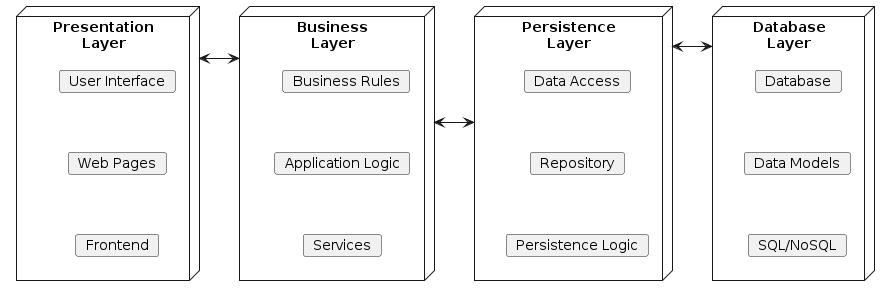
\includegraphics[width=\textwidth]{../../images/out/layered_architecture.png}

		\label{fig:layered_architecture}
	\end{figure}
\end{frame}

\begin{frame}
	\frametitle{Layered Architecture Topology}
	\begin{columns}[t]
		\column{0.5\textwidth}
		\begin{itemize}
			\item Follows a \textbf{four-layered architecture} that organizes software into distinct layers.
			\item Benefits include:
			\begin{itemize}
				\item Separation of concerns.
				\item Improved maintainability.
				\item Enhanced scalability and flexibility.
			\end{itemize}
		\end{itemize}
		\column{0.5\textwidth}
		\begin{itemize}
			\item \textbf{Common topology:}
			\begin{itemize}
				\item Presentation Layer.
				\item Business Layer.
				\item Persistence Layer.
				\item Database Layer.
			\end{itemize}
			\item \textbf{Other instances include:}
			\begin{itemize}
				\item Containerized Architecture (App Layer, Docker Layer, Host OS Layer, Infrastructure Layer).
				\item OSI Model (Application Layer, Presentation Layer, Session Layer).
				\item Microkernel Architecture (Core Layer, Extension Layer).
			\end{itemize}
		\end{itemize}
	\end{columns}
\end{frame}


\begin{frame}
	\frametitle{Presentation Layer}
	\begin{itemize}
		\item \textbf{Role and Function:}
		\begin{itemize}
			\item Manages interaction between the user and the system.
			\item Presents information to the user and receives user input.
		\end{itemize}
		\item \textbf{Context in Web Applications:}
		\begin{itemize}
			\item Includes elements such as web pages, user interfaces, and frontend logic.
		\end{itemize}
		\item \textbf{Key Components:}
		\begin{itemize}
			\item \textbf{User Interface (UI):} Direct interaction elements (buttons, forms, etc.).
			\item \textbf{Web Pages:} Frontend pages like home pages, dashboards, and submission forms.
			\item \textbf{Frontend:} Technologies (JavaScript, CSS, HTML) and frameworks (React, Angular).
		\end{itemize}
		\item \textbf{Communication:}
		\begin{itemize}
			\item Interacts with the Business Layer to fetch or send data based on user actions.
		\end{itemize}
	\end{itemize}
\end{frame}


\subsection{Business Layer}

\begin{frame}
	\frametitle{Business Layer Overview}
	\begin{itemize}
		\item Also known as the \textit{Application Logic} or \textit{Domain Logic} layer.
		\item Houses the core functionality of the application.
		\item Implements business rules and logic that define how the application should behave.
		\item Encapsulates the decisions, processes, and actions driving the application.
	\end{itemize}
\end{frame}

\begin{frame}
	\frametitle{Key Components of the Business Layer}
	\begin{itemize}
		\item \textbf{Business Rules:}
		\begin{itemize}
			\item Define the core principles and rules (e.g., calculation methods, data validation).
		\end{itemize}
		\item \textbf{Application Logic:}
		\begin{itemize}
			\item Contains detailed rules and processes, such as handling user input and managing state transitions.
		\end{itemize}
		\item \textbf{Services:}
		\begin{itemize}
			\item Includes both external and internal service layers.
			\item Manages tasks like sending emails, processing payments, or handling sessions.
		\end{itemize}
	\end{itemize}
\end{frame}

\begin{frame}
	\frametitle{Role in the Overall Architecture}
	\begin{itemize}
		\item Acts as a mediator between the Presentation and Persistence layers.
		\item Applies business logic to decide which data to retrieve or modify based on user actions.
	\end{itemize}
\end{frame}

\subsection{Persistence Layer}

\begin{frame}
	\frametitle{Persistence Layer Overview}
	\begin{itemize}
		\item Manages data access and storage for the application.
		\item Defines how data is stored, retrieved, and updated using databases or other storage mechanisms.
		\item Allows the Business Layer to interact with data without handling low-level storage operations.
	\end{itemize}
\end{frame}

\begin{frame}
	\frametitle{Key Components of the Persistence Layer}
	\begin{itemize}
		\item \textbf{Data Access:}
		\begin{itemize}
			\item Handles interactions with data storage systems.
			\item Provides the necessary queries or commands for database operations.
		\end{itemize}
		\item \textbf{Repository:}
		\begin{itemize}
			\item Abstracts the retrieval, update, and deletion of data entities.
		\end{itemize}
		\item \textbf{Persistence Logic:}
		\begin{itemize}
			\item Governs how data is stored, ensuring consistency and retrievability.
		\end{itemize}
	\end{itemize}
\end{frame}

\begin{frame}
	\frametitle{Interaction with the Database Layer}
	\begin{itemize}
		\item Communicates with the Database Layer to store and retrieve data.
		\item Ensures efficient data management for the Business Layer.
	\end{itemize}
\end{frame}

\subsection{Database Layer}

\begin{frame}
	\frametitle{Database Layer Overview}
	\begin{itemize}
		\item The foundational layer for persistent data storage.
		\item Consists of the actual database system and data models representing the data structure.
		\item Responsible for ensuring data integrity, consistency, and security.
	\end{itemize}
\end{frame}

\begin{frame}
	\frametitle{Key Components of the Database Layer}
	\begin{itemize}
		\item \textbf{Database:}
		\begin{itemize}
			\item The system used to store application data (e.g., MySQL, PostgreSQL, MongoDB).
		\end{itemize}
		\item \textbf{Data Models:}
		\begin{itemize}
			\item Define the structure of the data (e.g., tables in relational databases or collections in NoSQL systems).
		\end{itemize}
		\item \textbf{SQL/NoSQL:}
		\begin{itemize}
			\item Refers to the type of database used, each with its own use cases and methodologies.
		\end{itemize}
	\end{itemize}
\end{frame}

\begin{frame}
	\frametitle{Data Persistence and Integrity}
	\begin{itemize}
		\item Provides persistent storage, ensuring data remains available even after the application shuts down or restarts.
		\item Maintains the integrity and security of the stored data.
	\end{itemize}
\end{frame}

\subsection{Layer Interactions}

\begin{frame}
	\frametitle{Layer Interactions Overview}
	\begin{itemize}
		\item \textbf{Presentation Layer:}
		\begin{itemize}
			\item Sends user input to the Business Layer, requesting operations or data retrieval.
		\end{itemize}
		\item \textbf{Business Layer:}
		\begin{itemize}
			\item Processes requests by applying business logic.
			\item Communicates with the Persistence Layer to retrieve or modify data.
		\end{itemize}
		\item \textbf{Persistence Layer:}
		\begin{itemize}
			\item Accesses the Database Layer to perform necessary data operations.
		\end{itemize}
		\item \textbf{Database Layer:}
		\begin{itemize}
			\item Provides the required data back to the Persistence Layer.
		\end{itemize}
	\end{itemize}
\end{frame}

\begin{frame}
	\frametitle{Data Flow and Separation of Concerns}
	\begin{itemize}
		\item Data flows from the Presentation Layer to the Business Layer, then to the Persistence and Database Layers, and back.
		\item This structure maintains a high degree of separation of concerns:
		\begin{itemize}
			\item Each layer handles a specific aspect of the application’s operation.
			\item Enhances maintainability, making it easier to modify or replace components without impacting the entire system.
		\end{itemize}
	\end{itemize}
\end{frame}

\section{Closed and Open Layer Architectures}

\begin{frame}
	\frametitle{Overview of Closed and Open Layer Architectures}
	\begin{itemize}
		\item \textbf{Role in Software Design:}
		\begin{itemize}
			\item Organizes the system's components using a layered approach.
		\end{itemize}
		\item \textbf{Closed Layers:}
		\begin{itemize}
			\item Limit interaction and accessibility between layers.
		\end{itemize}
		\item \textbf{Open Layers:}
		\begin{itemize}
			\item Allow greater interaction and accessibility between layers.
		\end{itemize}
		\item \textbf{Illustration:}
		\begin{itemize}
			\item The diagram below visualizes the concepts of closed and open layers.
		\end{itemize}
	\end{itemize}
\end{frame}

\begin{frame}
	\frametitle{Diagram: Closed and Open Layer Architectures}
	\begin{figure}[ht]
		\centering
		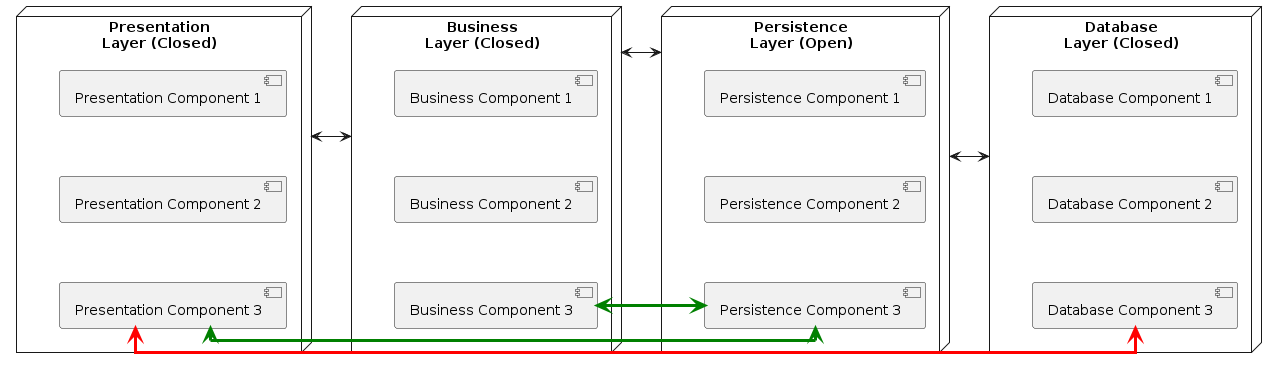
\includegraphics[width=\textwidth]{../../images/out/layered_architecture_open.png}
		\caption{Closed and Open Layer Architectures}
	\end{figure}
\end{frame}

\subsection{Closed Layer Architecture}

\begin{frame}
	\frametitle{Overview of Closed Layer Architecture}
	\begin{itemize}
		\item Layers where components interact only within the same layer or with adjacent layers.
		\item Direct external access to components is restricted.
		\item Provides security, stability, and encapsulation of logic.
	\end{itemize}
\end{frame}

\begin{frame}
	\frametitle{Components of Closed Layers}
	\begin{itemize}
		\item \textbf{Presentation Layer:}
		\begin{itemize}
			\item Contains \textit{Presentation Component 1}, \textit{Presentation Component 2}, and \textit{Presentation Component 3}.
			\item Components interact only with adjacent layers and not directly with external entities.
		\end{itemize}
		\item \textbf{Database Layer:}
		\begin{itemize}
			\item Comprises \textit{Database Component 1}, \textit{Database Component 2}, and \textit{Database Component 3}.
			\item Components are shielded from direct external modifications.
		\end{itemize}
	\end{itemize}
\end{frame}

\begin{frame}
	\frametitle{Prohibited Direct Connections}
	\begin{itemize}
		\item The red connection between \textit{Presentation Component 3} and \textit{Database Component 3} is prohibited.
		\item Direct communication between non-adjacent layers is not allowed.
		\item Any interaction between the Presentation and Database Layers must occur through the Persistence Layer.
		\item This rule enforces proper encapsulation and keeps system components well-separated.
	\end{itemize}
\end{frame}

\begin{frame}
	\frametitle{Examples of Closed Layer Architecture}
	\begin{itemize}
		\item \textbf{Banking Systems:}
		\begin{itemize}
			\item The Presentation Layer (e.g., web interfaces, mobile apps) and the Database Layer (e.g., user data, transaction records) remain isolated.
			\item Prevents direct interaction to mitigate the risk of data breaches.
		\end{itemize}
		\item \textbf{Healthcare Systems:}
		\begin{itemize}
			\item Patient data and treatment records in the Database Layer are not directly accessible by the Presentation Layer.
			\item All access goes through the Persistence Layer to enforce data validation, security, and privacy regulations.
		\end{itemize}
	\end{itemize}
\end{frame}

\subsection{Open Layer Architecture}

\begin{frame}
	\frametitle{Overview of Open Layer Architecture}
	\begin{itemize}
		\item Allows greater flexibility and external interaction.
		\item Exposes its components to communication from other layers.
		\item Enables data exchange and functional access across layers.
	\end{itemize}
\end{frame}

\begin{frame}
	\frametitle{Persistence Layer as an Open Layer}
	\begin{itemize}
		\item In the provided diagram, the Persistence Layer is designed as an open layer.
		\item Contains the following components:
		\begin{itemize}
			\item \textit{Persistence Component 1}
			\item \textit{Persistence Component 2}
			\item \textit{Persistence Component 3}
		\end{itemize}
		\item These components allow external interactions, particularly with other layers.
	\end{itemize}
\end{frame}

\begin{frame}
	\frametitle{Direct Interactions in Open Layers}
	\begin{itemize}
		\item \textit{Persistence Component 3} interacts directly with:
		\begin{itemize}
			\item \textit{Presentation Component 3}
			\item \textit{Business Component 3}
		\end{itemize}
		\item Green connections in the diagram illustrate these direct interactions.
		\item This design prioritizes flexibility and performance over strict encapsulation.
	\end{itemize}
\end{frame}

\begin{frame}
	\frametitle{When to Use Open Layer Architecture}
	\begin{itemize}
		\item \textbf{Performance Considerations:}
		\begin{itemize}
			\item In performance-sensitive applications (e.g., real-time systems), reducing latency is critical.
			\item Direct access by the Presentation or Business Layers can bypass intermediary overhead.
		\end{itemize}
		\item \textbf{Lack of Security Concerns:}
		\begin{itemize}
			\item Suitable for controlled environments (e.g., internal tools or non-sensitive systems).
			\item Direct communication is acceptable when security risks are minimal.
		\end{itemize}
	\end{itemize}
\end{frame}

\section{Advantages and Disadvantages of Layered Architecture}

\begin{frame}
	\frametitle{Overview}
	\begin{itemize}
		\item Layered architecture separates a system into distinct layers, each with specific functionality.
		\item This design supports modular development, better organization, and easier maintenance.
		\item However, it also comes with certain advantages and disadvantages.
	\end{itemize}
\end{frame}

\subsection{Advantages of Layered Architecture}

\begin{frame}
	\frametitle{Advantages of Layered Architecture (Part 1)}
	\begin{itemize}
		\item \textbf{Separation of Concerns:}
		\begin{itemize}
			\item Each layer is responsible for a specific aspect (e.g., presentation, business logic, data persistence).
			\item Improves readability and reduces complexity.
		\end{itemize}
		\item \textbf{Modularity and Maintainability:}
		\begin{itemize}
			\item Isolates components into distinct layers.
			\item Changes in one layer can often be made independently of others.
			\item Promotes code reuse and simplifies maintenance.
		\end{itemize}
	\end{itemize}
\end{frame}

\begin{frame}
	\frametitle{Advantages of Layered Architecture (Part 2)}
	\begin{itemize}
		\item \textbf{Scalability:}
		\begin{itemize}
			\item Different layers can be scaled independently based on their load.
			\item For example, additional servers can be allocated to a high-traffic presentation layer.
		\end{itemize}
		\item \textbf{Testability:}
		\begin{itemize}
			\item Clear separation allows individual layers to be isolated and tested.
			\item Improves test coverage and reduces the risk of bugs.
		\end{itemize}
		\item \textbf{Flexibility in Technology Choices:}
		\begin{itemize}
			\item Different layers can employ different technologies and frameworks.
			\item Enables the use of the best tools suited for each layer's purpose.
		\end{itemize}
	\end{itemize}
\end{frame}


\subsection{Disadvantages of Layered Architecture}

\begin{frame}
	\frametitle{Disadvantages of Layered Architecture (Part 1)}
	\begin{itemize}
		\item \textbf{Performance Overhead:}
		\begin{itemize}
			\item Each additional layer adds a level of abstraction.
			\item Inter-layer communication can introduce latency, particularly in high-performance applications.
		\end{itemize}
		\item \textbf{Complexity in Simple Systems:}
		\begin{itemize}
			\item For smaller applications with limited functionality, multiple layers may add unnecessary complexity.
		\end{itemize}
		\item \textbf{Tight Coupling Between Layers:}
		\begin{itemize}
			\item Heavy dependencies between layers can force changes in multiple layers when one is modified.
		\end{itemize}
	\end{itemize}
\end{frame}

\begin{frame}
	\frametitle{Disadvantages of Layered Architecture (Part 2)}
	\begin{itemize}
		\item \textbf{Rigidity in Layering:}
		\begin{itemize}
			\item Strict separation may limit the system's adaptability to changing requirements.
			\item Bypassing a layer or modifying interactions can require significant refactoring.
		\end{itemize}
		\item \textbf{Difficulty in Managing Cross-Cutting Concerns:}
		\begin{itemize}
			\item Issues such as security, logging, and transaction management often span multiple layers.
			\item Managing these concerns can lead to redundant code or require special handling (e.g., aspect-oriented programming).
		\end{itemize}
	\end{itemize}
\end{frame}



\subsection{Advantages and Disadvantages of Closed Layer Architecture}

\begin{frame}
	\frametitle{Advantages of Closed Layer Architecture}
	\begin{itemize}
		\item \textbf{Security and Encapsulation:}
		\begin{itemize}
			\item Isolates layers to protect components from external access.
			\item Ensures that sensitive data or logic remains hidden from unauthorized entities.
		\end{itemize}
		\item \textbf{Stability:}
		\begin{itemize}
			\item Restricting communication to adjacent layers reduces the risk of unintended interactions.
			\item Minimizes errors or unexpected behaviors from external access.
		\end{itemize}
		\item \textbf{Maintainability:}
		\begin{itemize}
			\item Encapsulated components with limited access simplify making internal changes.
			\item Modifications in one layer have minimal impact on other parts of the system.
		\end{itemize}
	\end{itemize}
\end{frame}

\begin{frame}
	\frametitle{Disadvantages of Closed Layer Architecture}
	\begin{itemize}
		\item \textbf{Limited Flexibility:}
		\begin{itemize}
			\item Restricting communication to adjacent layers can limit the overall flexibility.
			\item Can complicate the introduction of new layers or the need for more direct interactions.
		\end{itemize}
		\item \textbf{Increased Complexity in Communication:}
		\begin{itemize}
			\item External components cannot directly interact with closed layers.
			\item Reliance on adjacent layers as intermediaries leads to more complex interaction patterns.
		\end{itemize}
		\item \textbf{Potential Performance Overhead:}
		\begin{itemize}
			\item Additional intermediary layers (e.g., the Persistence Layer) may introduce performance bottlenecks if not designed efficiently.
		\end{itemize}
	\end{itemize}
\end{frame}

\subsection{Advantages and Disadvantages of Open Layer Architecture}

\begin{frame}
	\frametitle{Advantages of Open Layer Architecture}
	\begin{itemize}
		\item \textbf{Increased Flexibility:}
		\begin{itemize}
			\item Open layers allow direct communication across different layers.
			\item Easier to introduce new components or integrate with external systems without excessive intermediaries.
		\end{itemize}
		\item \textbf{Improved Performance:}
		\begin{itemize}
			\item Eliminates the need for intermediaries.
			\item Reduces overhead from additional communication steps, enhancing overall performance.
		\end{itemize}
		\item \textbf{Simplified Communication:}
		\begin{itemize}
			\item Facilitates direct interaction and data exchange between components.
			\item Removes the complexity of routing through intermediary layers.
		\end{itemize}
	\end{itemize}
\end{frame}

\begin{frame}
	\frametitle{Disadvantages of Open Layer Architecture}
	\begin{itemize}
		\item \textbf{Security Risks:}
		\begin{itemize}
			\item Direct access can expose critical data or business logic.
			\item Increases vulnerability to unauthorized access.
		\end{itemize}
		\item \textbf{Reduced Encapsulation:}
		\begin{itemize}
			\item Exposes internal components.
			\item Compromises the integrity of the system’s design.
		\end{itemize}
		\item \textbf{Maintenance Challenges:}
		\begin{itemize}
			\item Increased external interactions complicate system maintenance.
			\item Changes in one layer can have unintended effects on others.
		\end{itemize}
	\end{itemize}
\end{frame}

\section{Summary}
\begin{frame}
	\frametitle{Summary}
	\begin{itemize}
		\item Modular, n-tier design with clear separation of concerns.
		\item Evolved from monolithic systems to modern distributed architectures.
		\item Common topology: Presentation, Business, Persistence, and Database Layers.
		\item Layer interactions support \textbf{maintainability}, \textbf{scalability}, and \textbf{parallel development}.
		\item Closed architectures ensure \textbf{security}, \textbf{stability}, and \textbf{encapsulation}.
			\begin{itemize}
				\item \textbf{Stability}: (\textit{Controlled Interaction} – limits communication to adjacent layers; \textit{Predictable Behavior} – ensures well-defined interfaces; \textit{Fault Containment} – isolates errors within a layer; \textit{Maintenance Efficiency} – localizes updates to minimize impact)
			\end{itemize}
		\item Open architectures offer \textbf{flexibility}, \textbf{performance}, and \textbf{direct communication}.
		\item Trade-offs include potential performance overhead and increased complexity.
	\end{itemize}
\end{frame}

\end{document}
